\subsection{Планетарные туманности}

\begin{wrapfigure}[15]{r}{0.3\tw}
    \vspace{-1pc}
    \centering
    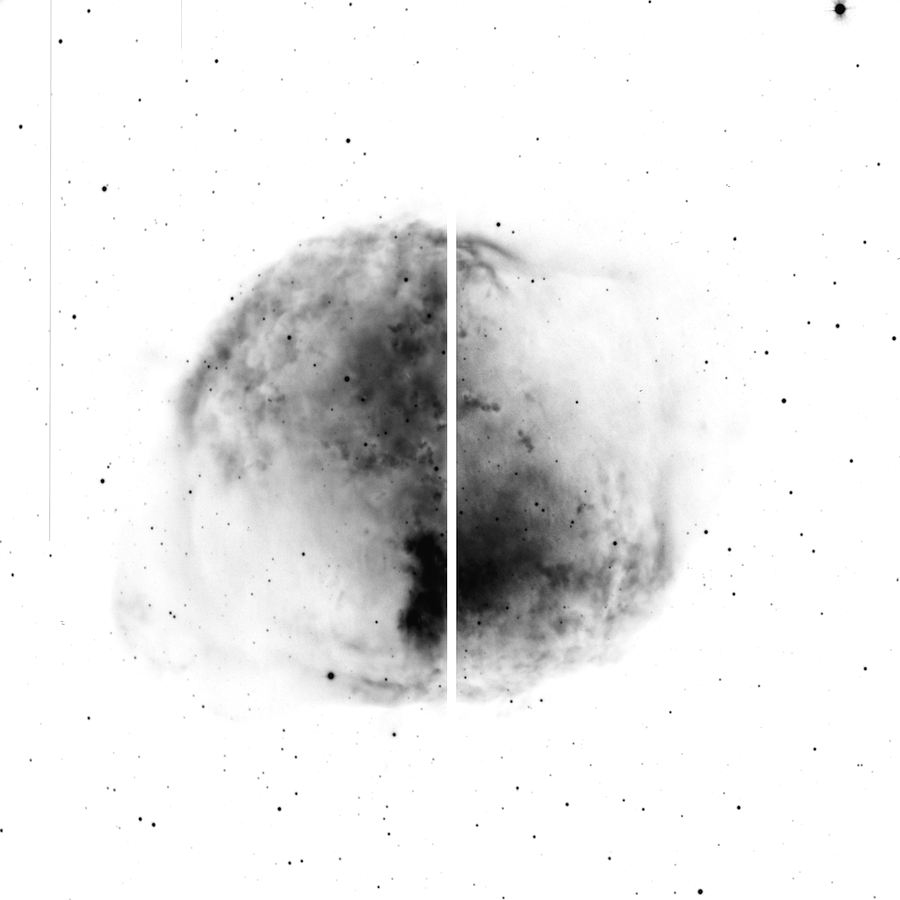
\includegraphics[width = 0.3\tw]{m27.png}
    \caption{Пла\-не\-тар\-ная туманность M27 (негатив). КГО, 2.5-метровый телескоп. Фильтры B, O\,III и $\text{H}_\alpha$. Чёрная полоса~--- артефакт матрицы, состоящей из двух чипов}
\end{wrapfigure}
\term{Планетарная туманность}~--- финальная стадия эволюции звезды средней массы, от $0.8M_\odot$ до $8M_\odot$. В процессе эволюции такие звезды становятся красными гигантами, в запускается процесс термоядерного синтеза более тяжёлых элементов~--- углерода и кислорода из гелия, но масса не достаточно, чтобы этот процесс был стабилен. И в итоге мощных пульсаций значительная масса вещества звезды выбрасывается в космическое пространство.  Но температуры ядра все ещё достаточно, чтобы ионизировать это вещество и заставить его излучать. Так облако выброшенного вещества становится планетарной туманностью.

Выброшенное вещество разлетается со скоростью несколько десятков километров в секунду. В то время, как оставшаяся звезда постепенно остывает, переставая ионизировать облако сброшенного вещества, и становится белым карликом. Облако рекомбинирует~--- становится нейтральным и перестает излучать. От момента взрыва звезды до рекомбинации проходит порядка 10000~лет, откуда несложно оценить, что характерный размер планетарной туманности составляет порядка 1~светового года.
 
 % http://www.astrosurf.com/buil/us/mission2/mission2.htm
\begin{figure}[h!]
    \centering
    \tikzsetnextfilename{spectrum-m27}
    \begin{tikzpicture}
        \footnotesize
        \begin{axis} [
            height = 4cm,
            width  = \tw,
            xlabel = {$\lambda,~\mathring{\text{A}}$},
            ylabel style={
                text width=3cm,
                align=center
            },
            ylabel = Относительная\\интенсивность,
            xmax   = 7000,
            xmin   = 4000,
            ytick  = {0, 1},
        ]
            \addplot[smooth] table[x=wavelength, y=intensity, col sep=comma]{data/spectrum-m27.txt};
            \draw[thin] (axis cs:6560,0.3) -- (axis cs:6400,0.5) node[anchor=south] {$\text{H}_\alpha$};
            \draw[thin] (axis cs:4861,0.12) -- (axis cs:4800,0.4) node[anchor=south] {$\text{H}_\beta$};
            \draw[thin] (axis cs:4340,0.07) -- (axis cs:4340,0.25) node[anchor=south] {$\text{H}_\gamma$};

            \draw[thin] (axis cs:4990,0.5) -- (axis cs:4850,0.7);
            \draw[thin] (axis cs:4959,0.37) -- (axis cs:4850,0.7) node[anchor=south] {O\,III};

            \draw[thin] (axis cs:6544,0.09) -- (axis cs:6530,0.8);
            \draw[thin] (axis cs:6581,0.22) -- (axis cs:6530,0.8) node[anchor=south] {N\,II};

            \draw[thin] (axis cs:4685,0.08) -- (axis cs:4600,0.3) node[anchor=south] {He\,II};
        \end{axis}
    \end{tikzpicture}
    \caption{Спектр планетарной туманности М27. Данные britastro.org}
    % http://www.astrosurf.com/buil/us/mission2/mission2.htm
    % https://britastro.org/specdb/data_graph.php?obs_id=86&obs_validated=1&obs_observer_id=DDB&r_c=1&f_c=0&o_comment=&plot=Plot
    % https://britastro.org/specdb/data.php
    \label{pic:spectrum-m27}
\end{figure}
 
 Спектр планетарной туманности состоит из эмиссионных линий тех элементов, из которых она состоит. Как было сказано выше, звезда сбрасывает оболочку уже после запуска синтеза тяжелых элементов из гелия. Одним из путей такого синтеза является CNO-цикл, на различных стадиях которого образуется, соответственно, углерод, азот и кислород. Ионизационное излучение которых можно наблюдать на спектре, например, \lookPicRef{pic:spectrum-m27}.
 
 
